%==============================================================================
% Compute-Aware Mixture-of-Experts for Efficient 5G Neural Receivers
% KNN project report, FIT BUT
% Stripped fitthesis frontmatter (no abstract/keywords/declaration/supervisor),
% kept the VUT title page styling.
% Authors: Dominik Huml (xhumld00), Jakub Kontrik (xkontr02), Martin Vaculik (xvaculm00)
%==============================================================================
\documentclass[english]{fitthesis}

\renewcommand{\rmdefault}{lmr}
\renewcommand{\sfdefault}{qhv}
\renewcommand{\ttdefault}{lmtt}

\csdoublequotesoff

\usepackage{url}
\usepackage{booktabs}
\usepackage{array}
\usepackage{multirow}
\usepackage{amsmath}
\usepackage{amssymb}
\usepackage{siunitx}

\ifWis
\ifx\pdfoutput\undefined
\else
  \usepackage{color}
  \usepackage[unicode,colorlinks,hyperindex,plainpages=false,pdftex]{hyperref}
  \definecolor{hrcolor-ref}{RGB}{223,52,30}
  \definecolor{hrcolor-cite}{HTML}{2F8F00}
  \definecolor{hrcolor-urls}{HTML}{092EAB}
  \hypersetup{
    linkcolor=hrcolor-ref,
    citecolor=hrcolor-cite,
    filecolor=magenta,
    urlcolor=hrcolor-urls
  }
  \def\pdfBorderAttrs{/Border [0 0 0] }
  \pdfcompresslevel=9
\fi
\else
\ifx\pdfoutput\undefined
\else
  \usepackage{color}
  \usepackage[unicode,colorlinks,hyperindex,plainpages=false,pdftex,urlcolor=black,linkcolor=black,citecolor=black]{hyperref}
  \definecolor{links}{rgb}{0,0,0}
  \definecolor{anchors}{rgb}{0,0,0}
  \def\AnchorColor{anchors}
  \def\LinkColor{links}
  \def\pdfBorderAttrs{/Border [0 0 0] }
  \pdfcompresslevel=9
\fi
\fi
\usepackage[all]{hypcap}

% Render \paragraph as a display heading (own line, then body below)
% instead of the default run-in style.
\usepackage{titlesec}
\titleformat{\paragraph}[block]
  {\normalfont\bfseries}{}{0pt}{}
\titlespacing*{\paragraph}{0pt}{1.2\baselineskip}{0.3\baselineskip}

% Title-page metadata. The VUT logo and faculty styling are kept.
% Abstract, keywords, declaration are not used in this project report.
\projectinfo{
  project={SP},
  year={2026},
  date=\today,
  title.cs={Compute-Aware MoE for Efficient 5G Neural Receivers},
  title.en={Compute-Aware MoE for Efficient 5G Neural Receivers},
  author.name={\shortstack[l]{Dominik Huml (xhumld00) \\ Jakub Kontrik (xkontr02) \\ Martin Vaculik (xvaculm00)}},
  author.surname={},
  department={UPGM},
  faculty={FIT},
  faculty.cs={Fakulta informačních technologií},
  faculty.en={Faculty of Information Technology},
  department.cs={Ústav počítačové grafiky a multimédií},
  department.en={Department of Computer Graphics and Multimedia},
  keywords.cs={},
  keywords.en={},
  abstract.cs={},
  abstract.en={},
  declaration={},
  tocdepth={2}
}

% Override fitthesis defaults: this is a KNN course project, not a standard
% "term project", and there is no supervisor row.
\makeatletter
\def\@projecttype@EN{KNN project}
\def\@projecttype@CS{KNN projekt}
\def\@projecttype@SK{KNN projekt}
\def\@supervisor@EN{}
\def\@supervisor@CS{}
\def\@supervisor@SK{}
\def\get@supervisor{}
\def\@supervisor@n{}
\def\@supervisor@s{}
\makeatother

\clubpenalty=10000
\widowpenalty=10000

\newlist{checklist}{itemize}{1}
\setlist[checklist]{label=$\square$}

% Suppress the abstract page and the declaration/acknowledgement page.
% The fitthesis \maketitle calls these internally for the thesis frontmatter.
% We are writing a paper, not a thesis.
\makeatletter
\renewcommand\makeabstract{}
\renewcommand\makedeclaration{}
\makeatother

\begin{document}
  \maketitle

  % Compute-Aware MoE for 5G Neural Receivers
% Single chapter with 6 sections.
% Run-ID and JSON traceability for every claim is in runs.md.

\chapter{Compute-Aware MoE for 5G Neural Receivers}
\label{chap:main}

\section{Introduction}
\label{sec:intro}

A 5G physical-layer receiver maps a received OFDM resource grid to soft bit estimates that an outer LDPC decoder corrects into the transmitted block. Recent work has shown that fully-neural receivers can match or surpass classical pipelines, particularly under hardware impairments and fast-varying channels~\cite{honkala2021deeprx,wiesmayr2024nrx}. Their drawback is uniform compute. Every slot pays the same cost regardless of channel quality, although many slots are comparatively easy while a smaller set of difficult slots dominates the residual error rate.

Mixture-of-Experts (MoE) architectures~\cite{shazeer2017outrageously,fedus2022switch} provide a mechanism for per-sample adaptive compute. A router selects a subset of experts to run for each input. Prior work on MoE for 5G receivers, MEAN~\cite{vanbolderik2024mean}, showed hard-gated adaptation for SIMO neural receivers. Related wireless MoE work has used channel conditions in the gating decision~\cite{song2025channelaware}. Together, these results support expert routing as a natural mechanism for channel-dependent computation.

Our contribution is a compute-aware neural receiver that combines (i) heterogeneous experts, (ii) a channel-aware router driven by shared-stem features with no oracle SNR access, and (iii) an explicit FLOPs penalty in the training loss. The primary metric is the \emph{BLER vs Average FLOPs} Pareto frontier on a held-out test set. We train and evaluate on synthetic 3GPP UMa and TDL-C channels generated with NVIDIA Sionna~\cite{sionna}, using \num{128} subcarriers, \num{14} OFDM symbols, 16-QAM, and four receive antennas.

\section{Related Work}
\label{sec:related}

\paragraph{Neural receivers for 5G}
DeepRx~\cite{honkala2021deeprx} and NRX~\cite{wiesmayr2024nrx} establish that fully-neural physical-layer receivers can match or surpass classical pipelines, particularly under hardware impairments and fast-varying channels. Both apply a single dense network uniformly to every slot, which motivates our compute-aware comparison.

\paragraph{Mixture-of-Experts for wireless}
The most relevant prior work for our setting is MEAN~\cite{vanbolderik2024mean}, a hard-gated MoE for a SIMO neural receiver. It demonstrates runtime adaptation and reports reduced active layers. Our work focuses on a different axis: we train heterogeneous experts (nano, small, large at $320$, $695$, and $1\,604$\,M FLOPs) with a stem-based router and an explicit FLOPs penalty, which lets us trace a BLER-FLOPs Pareto frontier (Section~\ref{sec:recipe}). Song et al.~\cite{song2025channelaware} study channel-aware gating for distributed wireless MoE, where link conditions influence expert selection. We use the same broad principle with receiver-side features inferred by the shared stem.

\paragraph{Mixture-of-Experts training mechanics}
The sparse expert formulation is from Shazeer et al.~\cite{shazeer2017outrageously}, with the Switch Transformer~\cite{fedus2022switch} contributing hard top-1 routing and a load-balance auxiliary. Differentiable routing uses Gumbel-Softmax~\cite{jang2017gumbel} with annealed temperature. Section~\ref{sec:recipe} tests these common anti-collapse mechanisms.

\paragraph{Simulators and data}
Synthetic 3GPP UMa and TDL-C training and test data are generated with NVIDIA Sionna~\cite{sionna}. The DeepMIMO~\cite{deepmimo} ASU Campus 1 ray-traced scenario provides the out-of-distribution test set used in Section~\ref{sec:scope}.

\section{Architecture}
\label{sec:arch}

The model has three components. A shared stem extracts channel-quality features, a channel-aware router picks one expert per sample, and three heterogeneous expert heads produce bit log-likelihood estimates. Figure~\ref{fig:arch} shows the layout.

Each slot is a $128 \times 14$ resource grid encoded as $16$ input channels from received samples and LS channel estimates, using real and imaginary parts over four antennas. The model appends two pilot-distance maps and outputs $4 \times 128 \times 14 = 7168$ bit LLRs, evaluated as BLER after decoding.

\begin{figure}[h]
\centering
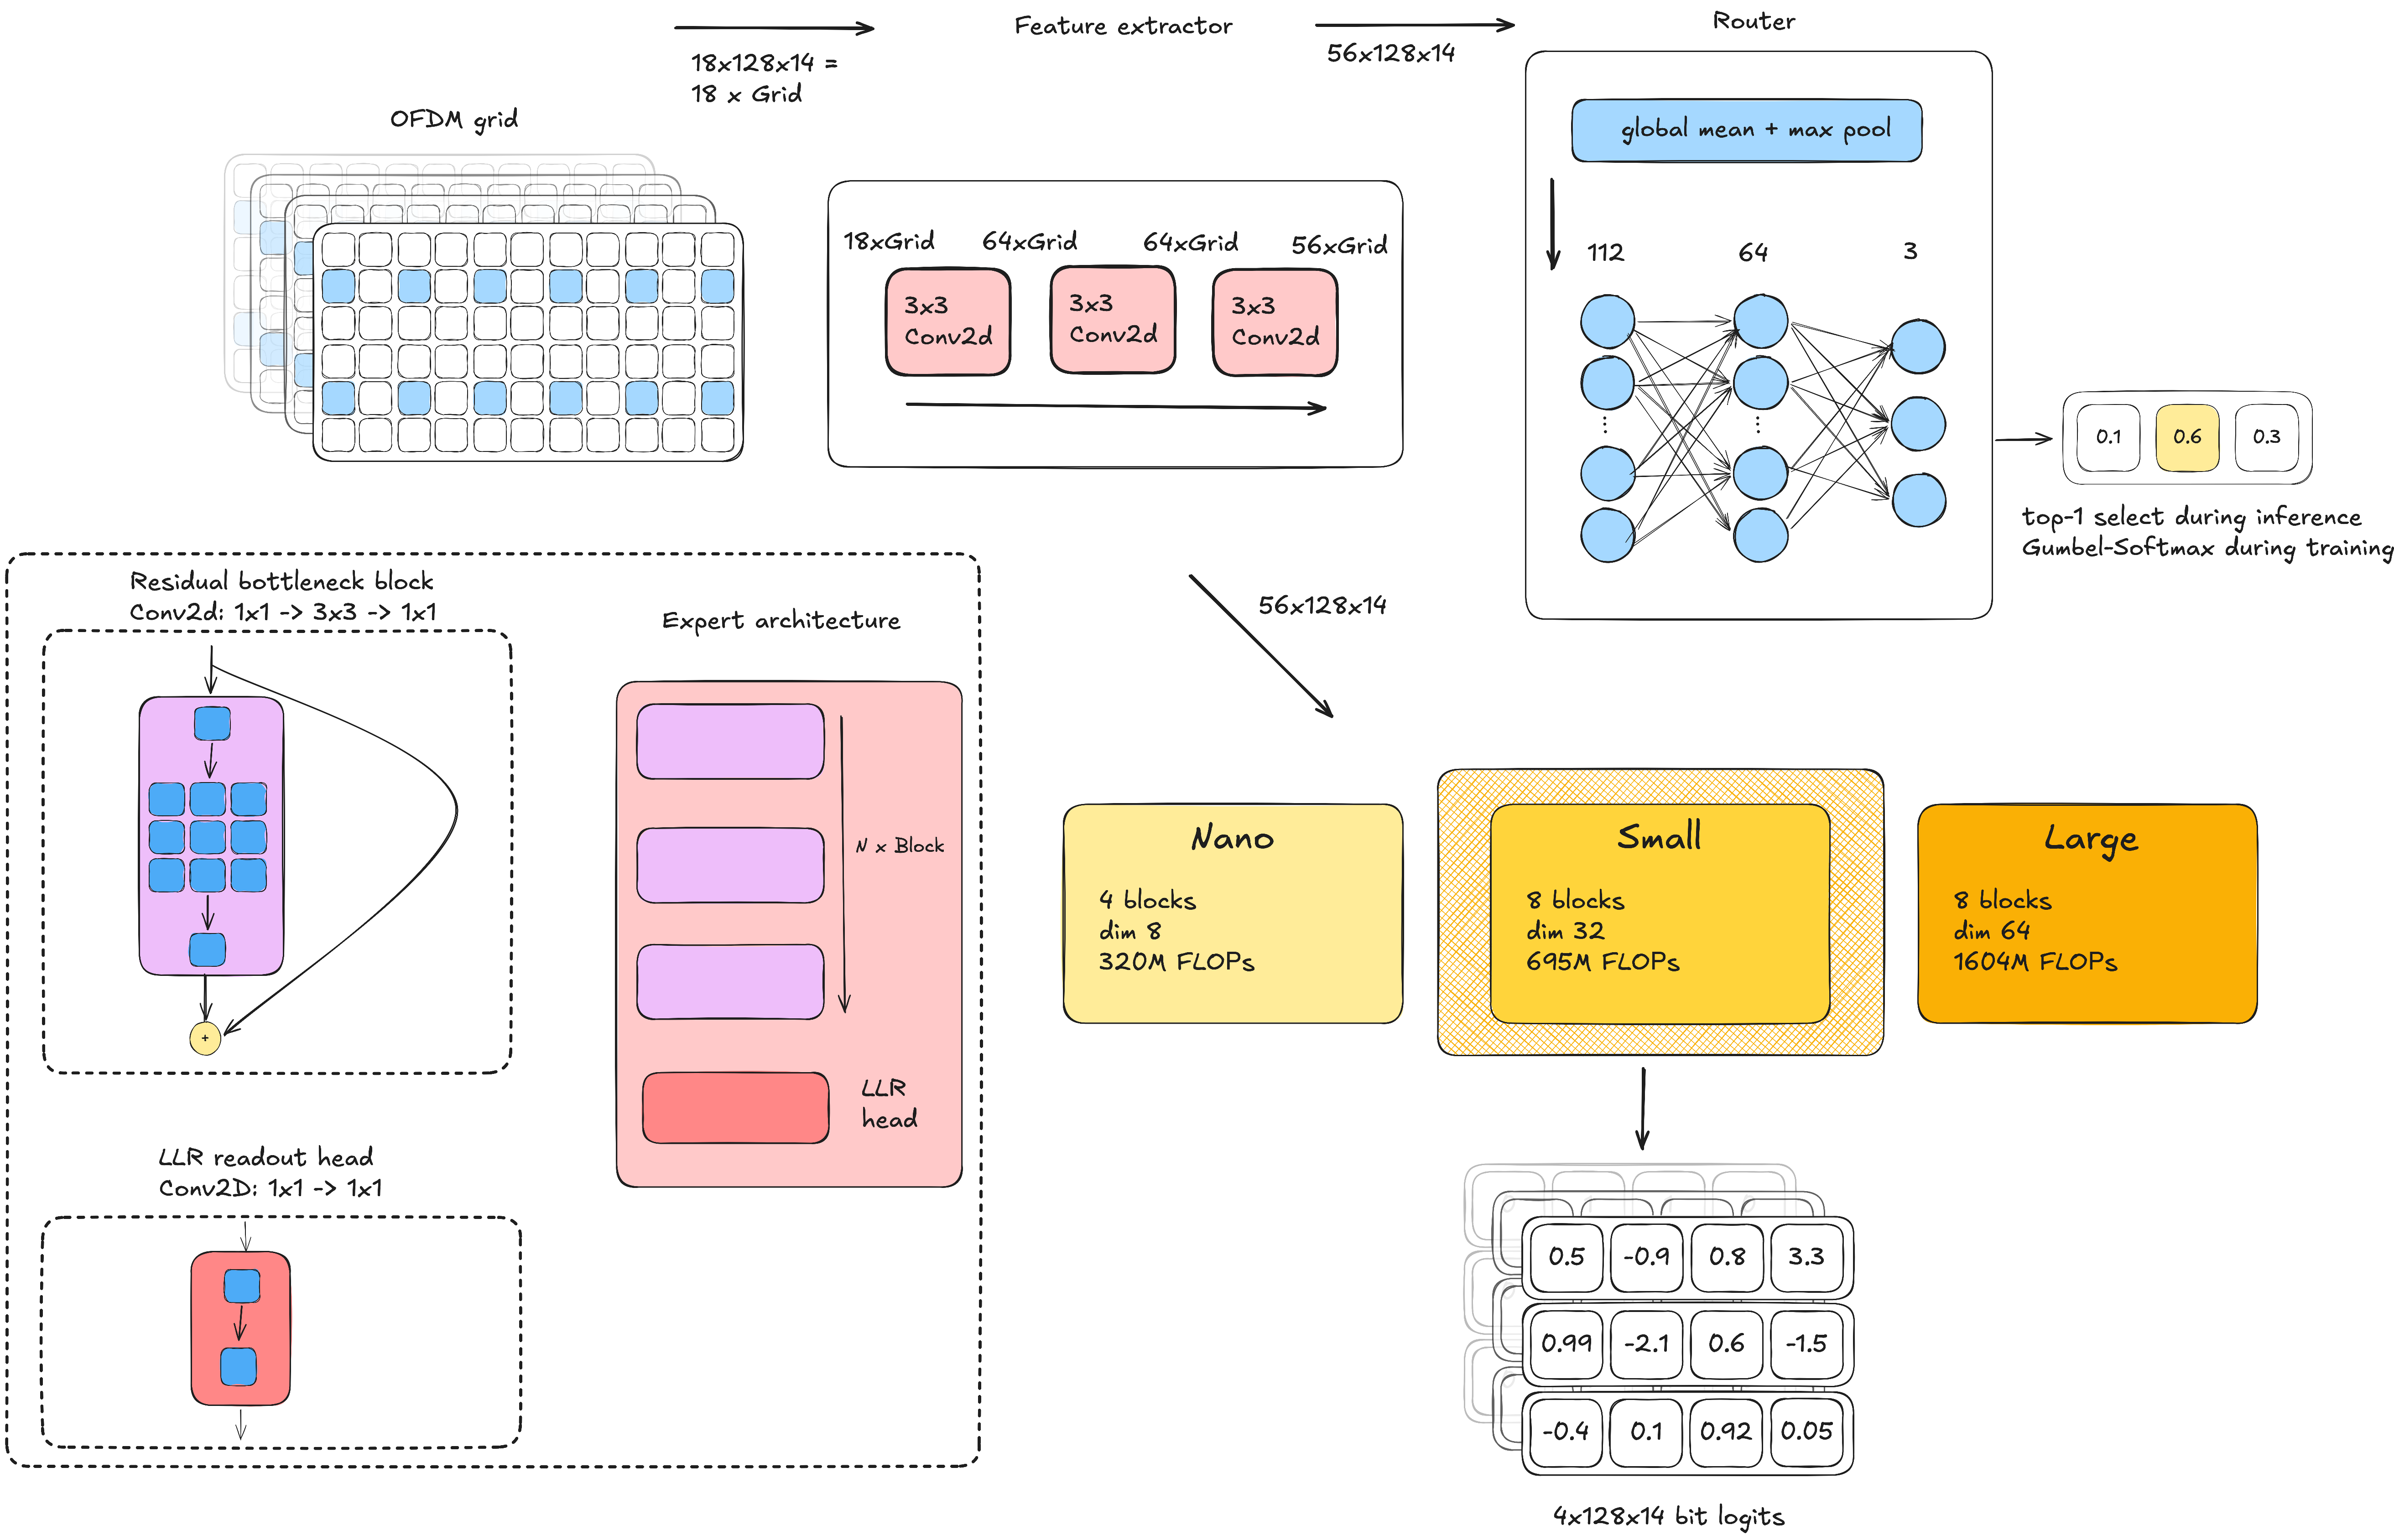
\includegraphics[width=0.95\linewidth]{obrazky-figures/architecture.pdf}
\caption{Compute-aware MoE neural receiver. The shared stem is always paid. The router selects exactly one expert per sample at inference. Experts have heterogeneous capacities ($1604$\,M, $695$\,M, and $320$\,M total FLOPs).}
\label{fig:arch}
\end{figure}

\paragraph{Shared stem}
A three-layer 2D~CNN with channels $18 \to 64 \to 64 \to 56$ and $3{\times}3$ convolutions maps the per-resource-element tensor to \texttt{state\_dim=56}. Two extra input channels carry pilot-distance features for LS channel-estimate interpolation. The stem costs $285$\,M multiply-add FLOPs per slot.

\paragraph{Channel-aware router}
A two-layer MLP ($112 \to 64 \to 3$, ReLU) maps mean-pooled and max-pooled stem features to expert logits. Training uses Gumbel-Softmax~\cite{jang2017gumbel} with temperature annealed from $1.0$ to $0.5$. At inference the router selects exactly one expert with hard top-1 and has no access to the true SNR.

\paragraph{Heterogeneous experts}
Each expert is a stack of residual bottleneck blocks ($1{\times}1 \to 3{\times}3 \to 1{\times}1$), followed by a bit-LLR readout head and a channel-estimate readout head. The three configurations are listed in Table~\ref{tab:experts}.

\begin{table}[h]
\centering
\small
\setlength{\tabcolsep}{6pt}
\begin{tabular}{l r r r r r}
\toprule
Expert & Blocks & Block dim & Readout dim & Total FLOPs & \% of large \\
\midrule
nano  & 4 &  8 &  32 & $320$\,M &  20\,\% \\
small & 8 & 32 &  96 & $695$\,M &  43\,\% \\
large & 8 & 64 & 128 & $1604$\,M & 100\,\% \\
\bottomrule
\end{tabular}
\caption{Heterogeneous expert configurations. \emph{Total FLOPs} is the sum of the always-paid stem ($285$\,M), the expert backbone, and the two readout heads. Values verified analytically and against the model's logged \texttt{max\_flops} buffer to within $0.01$\,\%.}
\label{tab:experts}
\end{table}

The complete model has $\num{582655}$ trainable parameters. Dense receivers at the corresponding capacity points ($\num{89892}$, $\num{168324}$, and $\num{449540}$ parameters) serve as baselines. The final recipe uses them to warm-start the stem and the \texttt{nano}/\texttt{small} experts in Section~\ref{sec:recipe}.

\paragraph{Training objective}
The loss combines the bit-level binary cross entropy with a channel-estimate auxiliary, an expected-FLOPs penalty, and a soft load-balance term,
\[
\mathcal{L} \;=\; \mathcal{L}_{\mathrm{BCE}}
  \;+\; \gamma \, \mathcal{L}_{\mathrm{chan}}
  \;+\; \alpha \, \mathbb{E}_{\mathrm{router}}\!\bigl[\,\widehat{C}\,\bigr]
  \;+\; \beta \, \mathcal{L}_{\mathrm{bal}},
\]
where $\widehat{C}$ is the total per-slot cost, stem included, normalised by the always-\texttt{large} receiver. We use $\gamma = 0.05$, $\alpha = 2 \cdot 10^{-3}$ at the final operating point, and $\beta = 0.1$. The expected-FLOPs term uses soft routing during training, while realised FLOPs use hard top-1 routing at inference.

\section{Training Recipe}
\label{sec:recipe}

Two degenerate regimes appear when training the compute-aware MoE. A cold start lets the FLOPs penalty push routing toward cheap experts before \texttt{large} can decode (BLER $0.926$ at $48\,\%$ FLOPs). A full warm-start gives \texttt{large} the initial advantage, yielding a fine-tuned dense receiver (BLER $0.879$ at $100\,\%$ FLOPs). Figure~\ref{fig:trajectories} contrasts these regimes with our asymmetric warm-start recipe.

\begin{figure}[h]
\centering
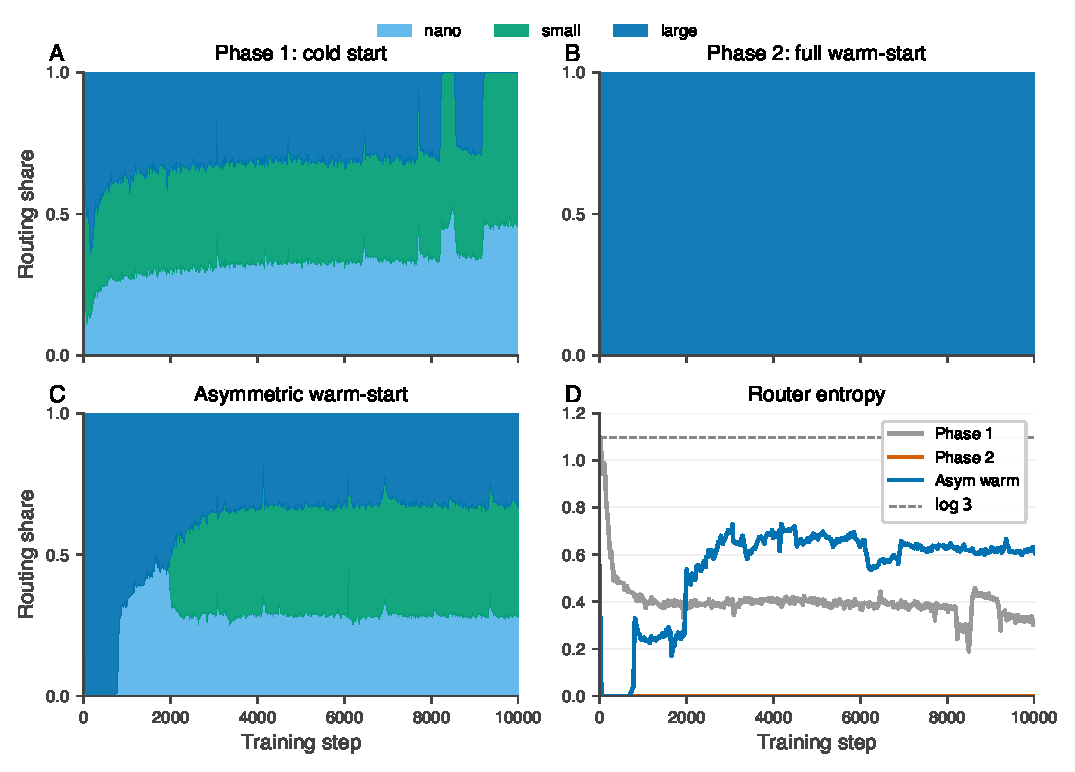
\includegraphics[width=0.95\linewidth]{obrazky-figures/routing_trajectories_collapse_modes.pdf}
\caption{Routing trajectories for the three paradigms. Phase~1 abandons \texttt{large} early, while Phase~2 converges to $100\,\%$ \texttt{large}. The asym-warm recipe (exp26) maintains exploratory router entropy long enough to reach a heterogeneous policy.}
\label{fig:trajectories}
\end{figure}

\paragraph{Anti-collapse mechanisms}
We tested four Switch auxiliary weights from $10^{-3}$ to $10^{0}$ and four soft capacity penalties from $0.1$ to $10.0$. None of the eight runs produced both heterogeneous routing and BLER in the exp26 range. The three smaller Switch weights collapsed to \texttt{large}. The largest weight spread soft probabilities, but hard top-1 routing still selected \texttt{large} for nearly all samples. A weak capacity penalty also collapsed, medium penalties spread routing but degraded average BLER by about $6$--$7$\,pp, and capacity weight $10.0$ recovered only a worse operating point than exp26. Two warmup variants gave the same conclusion. Large-warmup routed every tested seed to \texttt{large}, while $\beta$-warmup produced inconsistent routing and worse average BLER than the no-warmup baseline.

\paragraph{Asymmetric warm-start with cold-\texttt{large}.}
Our recipe warm-starts the stem, \texttt{nano}, and \texttt{small} from dense baselines while leaving \texttt{large} random. This removes the initial advantage that otherwise makes \texttt{large} dominate. In Figure~\ref{fig:wakeup}, cold \texttt{large} initially captures routing, \texttt{nano} catches up around step $\sim 1\,500$, \texttt{small} joins around $\sim 1\,700$, and from $\sim 3\,000$ onward all three experts remain active.

\begin{figure}[h]
\centering

\includegraphics[width=0.92\linewidth]{obrazky-figures/expert_usage_asym_warm.pdf}
\caption{Expert routing share (EMA) for exp26. Cold-initialised \texttt{large} dominates briefly at the start, then drops as the FLOPs penalty pushes the router toward the warm-started \texttt{nano} and \texttt{small}. From step $\sim 3\,000$ onward the routing is stably heterogeneous across all three experts.}
\label{fig:wakeup}
\end{figure}

\paragraph{Why cold-\texttt{large} specifically.}
Cold-\texttt{small} (exp56) produces heterogeneous routing but at higher cost (validation BLER $0.897$, FLOPs $67\,\%$). Cold-\texttt{nano} (exp57) routes essentially all samples to \texttt{large} (validation BLER $0.887$, FLOPs $100\,\%$). In this sweep, cold-\texttt{large} is the configuration that makes the router commit to smaller experts before \texttt{large} becomes competent.

\paragraph{The $\alpha$ sweep on the test set}
Table~\ref{tab:alpha} reports test-set BLER and average realised FLOPs for the four operating points (each $32\,768$ samples per profile). The knee of the Pareto curve sits at $\alpha = 2 \cdot 10^{-3}$.

\begin{table}[h]
\centering
\small
\setlength{\tabcolsep}{3pt}
\begin{tabular}{l c r r r l}
\toprule
Run & $\alpha$ & UMa BLER & TDLC BLER & Avg FLOPs & TDLC routing (l/n/s) \\
\midrule
Dense large baseline & n/a & $0.936$ & $0.866$ & $100\,\%$ & n/a \\
exp24 & $5{\cdot}10^{-4}$ & $0.936$ & $0.861$ & $100\,\%$ & $100/0/0$ \\
exp25 & $1{\cdot}10^{-3}$ & $0.938$ & $0.875$ & $56\,\%$ & $44/12/44$ \\
\textbf{exp26} & $\mathbf{2{\cdot}10^{-3}}$ & $\mathbf{0.937}$ & $\mathbf{0.867}$ & $\mathbf{56\,\%}$ & $\mathbf{44/15/40}$ \\
exp27 & $5{\cdot}10^{-3}$ & $0.940$ & $0.881$ & $60\,\%$ & $37/0/63$ \\
\bottomrule
\end{tabular}
\caption{Alpha sweep on the locked test set. Average realised FLOPs is taken over UMa+TDLC, normalised to the always-\texttt{large} cost ($1\,604$\,M). exp24 routes entirely to \texttt{large}. exp27 assigns no test samples to \texttt{nano}.}
\label{tab:alpha}
\end{table}

\paragraph{Channel-aware feature ablation}
Replacing the router input with fresh Gaussian noise raises test BLER to $0.968$ ($+6.6$\,pp) and sends $89\,\%$ of samples to \texttt{small} with $0\,\%$ \texttt{large} usage. This supports channel-quality input as the active mechanism, rather than the architecture or loss alone.

\paragraph{Linear probes indicate profile-specific channel features}
Linear probes on pooled stem features indicate profile-specific channel information. On TDL-C, SNR reaches $R^2 = 0.93$ and delay spread $R^2 = 0.65$. On UMa, the SNR probe is weaker ($R^2 = 0.42$), consistent with geometry-sensitive decodability. UMa-vs-TDL-C classification reaches $77.9\,\%$ accuracy.


\paragraph{Recipe stability is bimodal}
Re-running exp26 with seeds $\{32, 42\}$ gave one reproduction (s$42$, validation BLER $0.905$) and one degenerate run (s$32$, test BLER $0.958$, large abandoned). At $100$k samples, $\alpha = 2 \cdot 10^{-3}$ routes away from \texttt{large} for both s$67$ and s$42$. Scaling $\alpha$ down to $1 \cdot 10^{-3}$ (exp60) recovers exp26-quality at $100$k, with test BLER $0.9013$ at $58\,\%$ FLOPs. Recipe stability at fixed $\alpha$ remains open.

\section{Training-Scaffold Finding}
\label{sec:scaffold}

The exp26 model has three experts active in routing, but block-level success is concentrated entirely in the largest expert. This observation yields a deployment recipe that reduces FLOPs without retraining.

\paragraph{Per-expert success rate}
For each routed sample we record whether the assigned expert decoded the block. Across about $8\,000$ test samples, \texttt{nano} and \texttt{small} both succeed on $0\,\%$ of routed samples. Only \texttt{large} decodes successfully, on $23.2\,\%$ of UMa-routed samples ($n{=}1047$) and $29.4\,\%$ of TDL-C-routed samples ($n{=}1832$). Figure~\ref{fig:specialization} shows that routing is heterogeneous, but block success is not.

\begin{figure}[h]
\centering
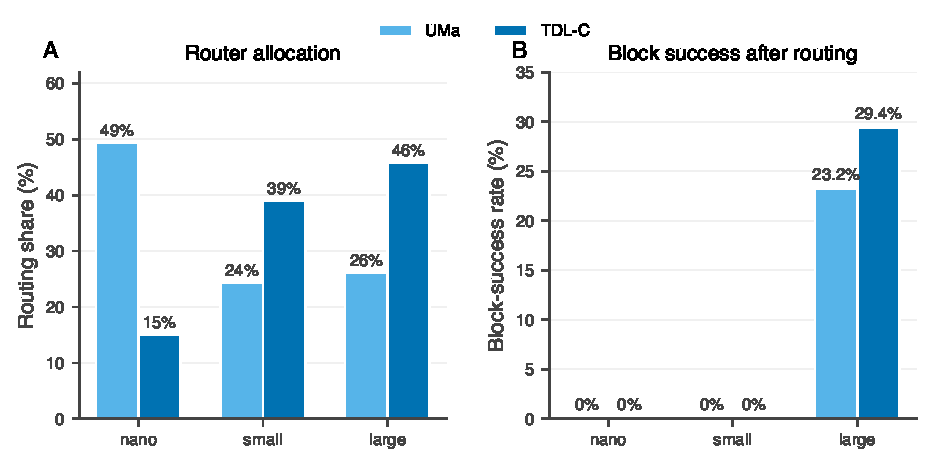
\includegraphics[width=\linewidth]{obrazky-figures/router_mechanism_expert_specialization.pdf}
\caption{The training-scaffold finding. The left panel shows that the router uses all three experts. The right panel shows that only \texttt{large} decodes routed samples successfully.}
\label{fig:specialization}
\end{figure}

\paragraph{Counterfactual decoding on \texttt{small}-routed samples}
For each test sample we forced every expert to decode it. On the UMa samples routed to \texttt{small} ($n{=}979$), pre-LDPC BER is nearly identical: \texttt{nano} $0.237$, \texttt{small} $0.230$, and \texttt{large} $0.231$. BLER is $1.000$ for all three. The router therefore sends this subset to \texttt{small} in a regime where no evaluated expert changes the block outcome. The routing decision reduces compute on samples that were not recovered by any evaluated expert, rather than recovering them through \texttt{small}.

\paragraph{Mode B substitutes \texttt{small} with a zero-output sink at inference.}
If \texttt{small}'s deployed BLER contribution is zero, its expert computation can be removed. We replace its expert head with a constant zero output and charge zero FLOPs whenever the router selects \texttt{small}. No retraining is performed.

\begin{table}[h]
\centering
\small
\setlength{\tabcolsep}{6pt}
\begin{tabular}{l c c c c c}
\toprule
 & \multicolumn{2}{c}{Avg BLER} & & \multicolumn{2}{c}{Avg FLOPs} \\
\cmidrule(lr){2-3}\cmidrule(lr){5-6}
Checkpoint & base & Mode B & $\Delta$ & base & \textbf{Mode B} \\
\midrule
exp25 ($\alpha\,{=}\,10^{-3}$)         & $0.9063$ & $0.9066$ & $+0.0003$ & $56.0\,\%$ & $\mathbf{46.7\,\%}$ \\
\textbf{exp26} ($\alpha\,{=}\,2{\cdot}10^{-3}$) & $\mathbf{0.9021}$ & $\mathbf{0.9021}$ & $\mathbf{0.0000}$ & $55.8\,\%$ & $\mathbf{47.3\,\%}$ \\
exp27 ($\alpha\,{=}\,5{\cdot}10^{-3}$)        & $0.9107$ & $0.9116$ & $+0.0009$ & $60.0\,\%$ & $\mathbf{41.9\,\%}$ \\
\bottomrule
\end{tabular}
\caption{Mode B inference. On the selected operating point (exp26) BLER is unchanged to four decimals, and FLOPs drops by $8.5$\,pp. Across all three $\alpha$ values BLER drift stays at or below $10^{-3}$.}
\label{tab:modeb}
\end{table}

Figure~\ref{fig:pareto} places these operating points against the dense neural ladder and the LS-MRC reference.

\begin{figure}[h]
\centering
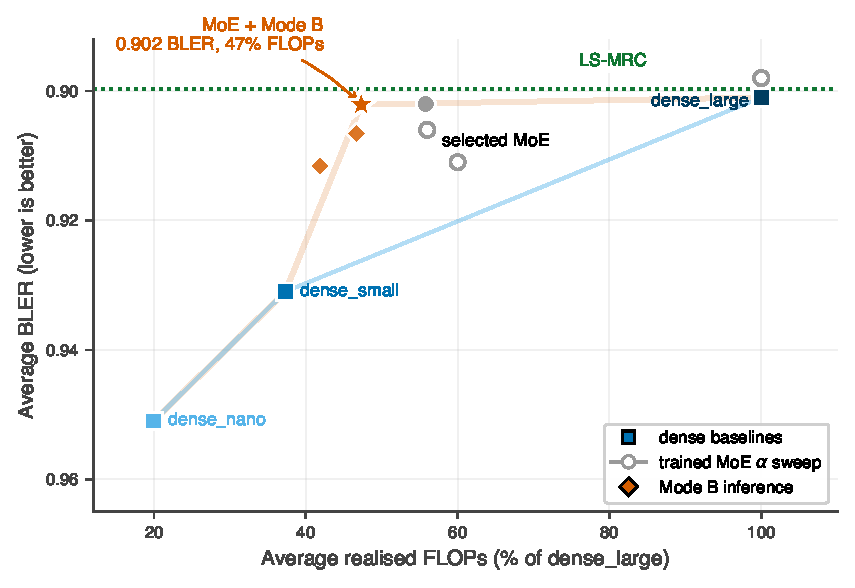
\includegraphics[width=0.92\linewidth]{obrazky-figures/report_pareto.pdf}
\caption{Pareto frontier on the locked test set. Dense neural baselines trade BLER for FLOPs. The trained MoE lands near dense\_large at $56\,\%$ FLOPs, while Mode B shifts it leftward. \textbf{exp26 + Mode B is within $0.002$ BLER of dense\_large at $47.3\,\%$ FLOPs.} LS-MRC is the classical reference and has no neural FLOPs.}
\label{fig:pareto}
\end{figure}

\paragraph{Why \texttt{small} is needed during training.}
exp41 drops \texttt{small} and trains $\{\texttt{nano}, \texttt{large}\}$ under the same recipe. Validation BLER rises to $0.955$, a $+5.3$\,pp loss against exp26's matched-protocol $0.902$. Removing \texttt{small} from training is therefore much more harmful than removing it at inference. The result indicates that \texttt{small} shapes the optimisation trajectory, even though its expert head is dispensable after training.

\paragraph{Role of \texttt{nano}.}
The symmetric ablation drops \texttt{nano} and trains only \texttt{small} and \texttt{large}. It gives test BLER $0.909$ at $65\,\%$ FLOPs, costing $+0.7$\,pp BLER and $+9$\,pp FLOPs versus exp26. Since \texttt{nano} absorbs many samples whose block outcome does not change under larger experts, dropping it costs more in compute than in BLER.

\paragraph{Training with a sink expert}
We also trained models with a zero-output expert from the start. The sink, channel-only, large variant ends at $82\,\%$ FLOPs. The sink, small, large variant moves to the all-sink solution by step $500$ and reaches BLER $1.0$. The sink, nano, large variant is stable but ends $7$\,pp BLER worse than exp26. The sink expert is therefore useful post hoc, but not as a trainable expert under the same recipe.

\paragraph{Deployment interpretation}
The resulting MoE is best understood as one decoding expert, \texttt{large}, plus cheaper routing outcomes for samples where extra capacity does not change the block result. \texttt{small} is useful during optimisation but removable at deployment. \emph{exp26 + Mode B} achieves BLER $0.9021$ at $47.3\,\%$ of dense-large FLOPs with no retraining.

\section{Scope and Discussion}
\label{sec:scope}

The contribution is positioned against dense neural receivers. We add scope checks against classical baselines, oracle routing, and ray-traced channels.

\paragraph{Full baseline landscape}
For a fair compute-vs-quality comparison we evaluated three classical baselines and three dense neural baselines of varying capacity on the same locked test set ($32\,768$ samples per profile). Table~\ref{tab:baselines} reports the full landscape.

\begin{table}[h]
\centering
\footnotesize
\setlength{\tabcolsep}{4pt}
\begin{tabular}{l l r r r r}
\toprule
Baseline & Channel info & Avg BLER & UMa & TDL-C & Avg FLOPs \\
\midrule
Single-antenna           & none      & $0.9950$ & $0.9922$ & $0.9978$ & n/a \\
Genie-MRC (oracle) & true H    & $\mathbf{0.8544}$ & $0.9084$ & $0.8003$ & n/a \\
LS-MRC             & LS pilots & $0.8997$ & $0.9388$ & $0.8607$ & n/a \\
\midrule
dense\_nano  & LS+net    & $0.951$  & $0.961$  & $0.941$  & $320$\,M \\
dense\_small & LS+net    & $0.931$  & $0.951$  & $0.911$  & $599$\,M \\
dense\_large & LS+net    & $0.901$  & $0.936$  & $0.866$  & $1604$\,M \\
\midrule
\textbf{exp26 + Mode B (ours)} & LS+net & $\mathbf{0.9021}$ & $0.937$ & $0.867$ & $\mathbf{759}$\,M \\
\bottomrule
\end{tabular}
\caption{All baselines on the same locked test set. Single-antenna is a no-MIMO floor. Genie-MRC needs oracle channel knowledge and is not deployable. LS-MRC is the realistic classical baseline. exp26 + Mode B is within $0.002$ BLER of dense\_large while using less than half of dense\_large's neural FLOPs.}
\label{tab:baselines}
\end{table}

exp26 + Mode B reaches dense\_large-level BLER at $\sim 47\,\%$ of dense\_large FLOPs. This is below half of the full neural receiver while remaining much more accurate than dense\_small. Against classical baselines it has much lower BLER than single-antenna detection and is essentially tied with LS-MRC on average BLER. The oracle Genie-MRC receiver has the lowest average BLER, so the comparison with classical receivers is channel-dependent. On the TDL-C waterfall, LS-MRC is uniformly better than both neural models between $14$ and $20$\,dB SNR (Table~\ref{tab:lmmse-snr}).


On three in-family OOD profiles (TDL-A, TDL-D, CDL-A), exp26 and dense\_large both average $0.825$, while LS-MRC averages $0.802$. The MoE preserves dense-neural quality while reducing neural compute, but the classical receiver has lower BLER on these profiles.

\paragraph{An oracle-SNR cascade is a tighter Pareto reference}
Beyond the dense ladder we compare against a hand-rule cascade using true SNR, an upper bound not deployable in practice. At tolerance $+0.01$--$0.02$ it reaches BLER $0.900$ at $49\,\%$ FLOPs, slightly dominating learned routing ($0.902$ at $56\,\%$). Looser tolerances reach $0.909$ at $34\,\%$ and $0.919$ at $27\,\%$. exp26 remains on the Pareto frontier without oracle SNR access. A direct SNR-statistics router ablation (exp38) collapsed to $100\,\%$ \texttt{large}.

\paragraph{Where neural receivers retain an advantage}
UMa shows the opposite pattern from TDL-C. The receivers tie within $1$\,pp at low and mid SNR, while neural decoders have slightly lower BLER at SNR $\geq 20.5$\,dB (Table~\ref{tab:lmmse-snr}). A UMa crosstab gives exp26 a net $+64$ block advantage over LS-MRC. On TDL-C, the same crosstab favours LS-MRC by $220$ blocks. The UMa NN-favoured subset has weaker MIMO geometry, with mean spatial max-eigenvalue $2.07$ against $3.22$ and channel power $0.56$ against $0.89$, suggesting that learned representations help when MRC aggregation is less favourable.

\begin{table}[h]
\centering
\small
\setlength{\tabcolsep}{5pt}
\begin{tabular}{c c c c | c c c c}
\toprule
\multicolumn{4}{c|}{TDL-C waterfall} & \multicolumn{4}{c}{UMa high-SNR} \\
SNR (dB) & LS-MRC & dense\_large & exp26 & SNR (dB) & LS-MRC & dense\_large & exp26 \\
\midrule
$14.0$--$15.5$ & $\mathbf{0.7050}$ & $0.7069$ & $0.7265$ & $14.5$--$16.0$ & $\mathbf{0.9047}$ & $0.9162$ & $0.9168$ \\
$15.5$--$17.0$ & $\mathbf{0.3213}$ & $0.3722$ & $0.3697$ & $17.5$--$19.0$ & $\mathbf{0.8443}$ & $\mathbf{0.8443}$ & $0.8449$ \\
$17.0$--$18.5$ & $\mathbf{0.1324}$ & $0.1850$ & $0.1745$ & $20.5$--$22.0$ & $0.8100$ & $0.7981$ & $\mathbf{0.7856}$ \\
$18.5$--$20.0$ & $\mathbf{0.0502}$ & $0.0698$ & $0.0851$ & $22.0$--$23.5$ & $0.7825$ & $\mathbf{0.7551}$ & $0.7651$ \\
                &                  &          &          & $23.5$--$25.0$ & $0.7629$ & $\mathbf{0.7320}$ & $0.7423$ \\
\bottomrule
\end{tabular}
\caption{Per-SNR BLER, $32\,768$ samples per profile. LS-MRC has lower TDL-C BLER throughout the plotted waterfall region, while neural receivers have lower UMa BLER at SNR $\geq 20.5$\,dB by $1$--$3$\,pp.}
\label{tab:lmmse-snr}
\end{table}

\paragraph{Out-of-distribution behaviour on ray-traced channels}
On DeepMIMO ASU Campus 1 ray-traced channels the neural decoders have near-unit BLER (dense\_large $0.9901$, exp26 $0.9915$), and exp26 falls back mostly to \texttt{nano} at $\sim 32\,\%$ FLOPs. In Figure~\ref{fig:pca-ood}, ASU samples form a tight off-centroid cluster in the in-distribution stem-feature PCA basis, with only $20\,\%$ inside the one-sigma box. A few-shot fine-tune ($2\,048$ samples, $500$ steps) did not recover. As a control, LS-MRC on DeepMIMO O1 reaches $0.976$ against dense\_large $0.982$ and exp26 $0.984$, suggesting a learned-prior mismatch rather than channel difficulty alone. Closing the gap requires longer fine-tuning, a larger OOD slice, or domain-randomised pre-training.

\begin{figure}[h]
\centering
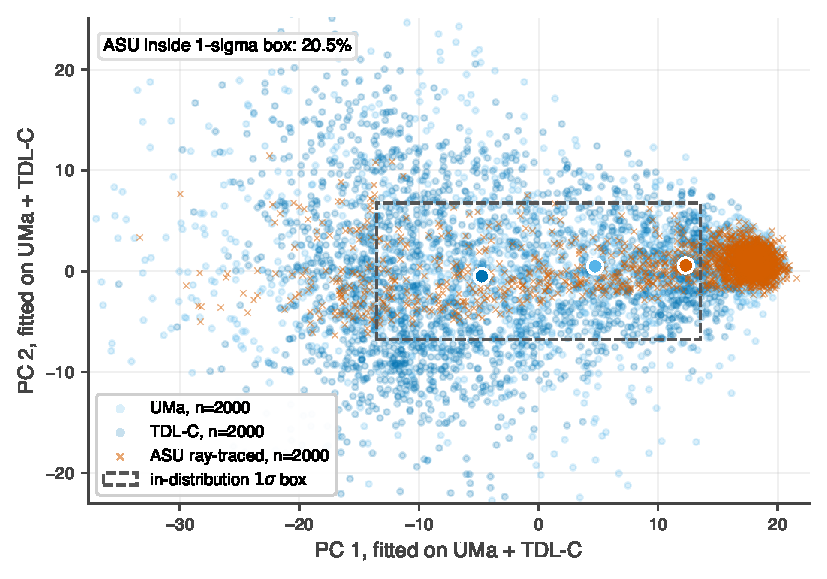
\includegraphics[width=0.78\linewidth]{obrazky-figures/pca_ood_overlay.pdf}
\caption{Stem-feature PCA-2D fitted on in-distribution UMa+TDL-C. ASU ray-traced samples (orange) projected onto the same basis collapse into a narrow off-centroid cluster (only $20\,\%$ inside the in-distribution one-sigma box), explaining the router's \texttt{nano} default on OOD.}
\label{fig:pca-ood}
\end{figure}

\paragraph{Conclusion}
We presented a compute-aware MoE neural receiver. Per-expert success analysis showed that the middle expert did not decode any block in the evaluated setting. Replacing it with a zero-output sink at inference preserves BLER to four decimals while saving $8.5$\,pp FLOPs, with no retraining. Diverse experts are needed during optimisation, but the non-decoding middle expert can be pruned at deployment. Open problems include recipe stability and OOD transfer to ray-traced channels.


\makeatletter
\def\@openbib@code{\addcontentsline{toc}{chapter}{Bibliography}}
\makeatother
\bibliographystyle{bib-styles/Pysny/enplain}

  \begin{flushleft}
  \bibliography{projekt-20-literatura-bibliography}
  \end{flushleft}

\end{document}
